\documentclass[11pt,letterpaper]{article}
\usepackage{graphicx, geometry, amsmath, amssymb, hyperref, natbib, booktabs, xcolor, listings}
\usepackage[export]{adjustbox}
\geometry{margin=1in}
\hypersetup{colorlinks=true, linkcolor=black, citecolor=black, urlcolor=black}

\title{Topology-Guided Feature Interaction Discovery via Persistent Homology:\\When Simplicial Complexes Illuminate but Do Not Improve Tabular Learning}

\author{Anonymous}

\date{}

\begin{document}

\maketitle

%-------------------------------------------------------------
\begin{abstract}
We investigate whether persistent homology---a tool from topological data analysis (TDA)---can discover and exploit higher-order feature interactions in tabular machine learning.
Inspired by simplicial complex models from opinion dynamics, where group interactions produce qualitatively different dynamics than pairwise projections, we propose Simplicial-Constrained Oblique Tree Sums (SC-OTS): a method that constructs a feature interaction simplicial complex via Vietoris--Rips persistent homology on target-aware distance correlation dissimilarity matrices, then uses this complex to constrain which features may combine in oblique splits of a FIGS-style greedy tree sum.
We evaluate SC-OTS on 10 tabular benchmarks (63,205 examples total) spanning synthetic datasets with ground-truth interactions and real-world datasets, comparing against FIGS, RO-FIGS, XGBoost, and EBM baselines.
Our results reveal a nuanced picture: the TDA-based interaction detection pipeline achieves the best F1 score (0.603) among five interaction detection methods on synthetic benchmarks with perfect faithfulness precision (1.0), and the simplicial complex provides a novel topological interpretability artifact.
However, two independent ablation studies---in both custom oblique trees and XGBoost---demonstrate that constraining model splits to the discovered simplicial complex does not improve predictive accuracy over unconstrained approaches (all Wilcoxon $p > 0.05$).
We conclude that persistent homology is a genuinely superior tool for discovering feature interactions compared to classical statistical methods, but its value lies in diagnostics and interpretation rather than architectural constraint.
We release our target-aware distance correlation pipeline and benchmark suite.
\end{abstract}

%-------------------------------------------------------------
\section{Introduction}
\label{sec:introduction}

Understanding how features interact is fundamental to building interpretable and accurate machine learning models for tabular data. While single-feature effects are well-captured by generalized additive models \citep{Lou2013, Caruana2015}, higher-order interactions---where three or more features jointly influence the target in ways not reducible to their pairwise effects---remain difficult to discover and exploit. Current approaches either detect interactions post hoc \citep{Lundberg2017, Tsang2020} or leave interaction discovery implicit in the tree-building process \citep{Breiman2001, Chen2016}.

In opinion dynamics research, simplicial complexes have demonstrated that simultaneous group interactions produce qualitatively different dynamics than their pairwise projections---including discontinuous phase transitions, bistability, and faster consensus that pairwise graph models cannot replicate \citep{Iacopini2019, Battiston2021}. This insight suggests a parallel in tabular machine learning: higher-order feature interactions may be first-class structural objects that should be explicitly discovered and modeled, not merely left to emerge from tree paths.

We propose Simplicial-Constrained Oblique Tree Sums (SC-OTS), a method that transfers the simplicial complex framework from opinion dynamics to feature interaction discovery in tabular learning. SC-OTS operates in three stages: (1) compute a pairwise feature dissimilarity matrix using target-aware distance correlation, (2) construct a Vietoris--Rips simplicial complex via persistent homology to identify robust multi-way feature interactions, and (3) constrain oblique splits in a FIGS-style \citep{Tan2022} greedy tree sum to only combine features that share a simplex. The simplicial complex itself serves as an interpretable ``interaction map'' that summarizes the higher-order interaction landscape.

Our investigation yields a carefully nuanced result. The TDA-based interaction detection pipeline genuinely outperforms classical methods: it achieves $\text{F1} = 0.603$ on synthetic benchmarks with ground-truth interactions, compared to 0.218 for ANOVA and 0.398 for tree-based detection, with perfect faithfulness precision (no false positive interactions). However, two rigorous ablation studies---in both custom oblique tree sums and XGBoost with interaction constraints---demonstrate that using the simplicial complex to constrain model architecture does not reliably improve predictive accuracy (all $p > 0.05$). The topological structure illuminates the interaction landscape but does not improve predictions on the benchmarks studied.

Our contributions are:
\begin{enumerate}
    \item A target-aware distance correlation pipeline for constructing metrically valid feature interaction simplicial complexes via persistent homology.
    \item Comprehensive empirical evidence across 10 datasets and 12 experimental artifacts that TDA-based interaction detection outperforms classical alternatives.
    \item Honest negative results from two independent ablation studies showing that topological constraints do not improve accuracy.
    \item The insight that simplicial complexes serve better as diagnostic and interpretive tools than as architectural constraints for tree-based models.
\end{enumerate}

%-------------------------------------------------------------
\section{Related Work}
\label{sec:related}

\paragraph{Interpretable tree ensembles.}
FIGS (Fast Interpretable Greedy-Tree Sums) \citep{Tan2022} generalizes CART by growing multiple trees simultaneously in an additive model, producing compact interpretable ensembles. RO-FIGS \citep{Matjasec2025} extends FIGS with oblique splits using linear combinations of random feature subsets and L1/2 regularization. Our work builds on this line by replacing random feature subset selection with topologically-guided subsets. XGBoost \citep{Chen2016} supports user-specified interaction constraints that restrict which features may appear together in tree branches; our approach automates this specification using persistent homology.

\paragraph{Generalized additive models and interaction detection.}
\citet{Lou2013} introduced GA2M, which learns pairwise interaction terms in intelligible models. \citet{Caruana2015} extended this to healthcare applications demonstrating the clinical value of interpretable pairwise interactions. The InterpretML framework \citep{Nori2019} implements EBMs (Explainable Boosting Machines) supporting up to 3-way interactions. While these methods explicitly model low-order interactions, they do not provide a topological characterization of the interaction landscape. Iterative Random Forests (iRF) \citep{Kumbier2018} detect high-order feature interactions by iteratively reweighting features in random forests, but as a post-hoc analysis step that does not constrain tree construction.

\paragraph{Neural interaction detection.}
\citet{Tsang2020} propose Neural Interaction Detection (NID), which uses learned neural network weights to identify statistical interactions between features. While NID can detect arbitrary-order interactions, it requires training a neural network and does not provide the topological invariants (Betti numbers, persistence diagrams) that characterize the global interaction structure.

\paragraph{Topological data analysis in machine learning.}
Persistent homology \citep{Zomorodian2005} has been applied to machine learning primarily as a feature engineering tool---extracting topological descriptors from data to serve as inputs to standard classifiers \citep{Pun2022}. The GUDHI library \citep{Maria2014} provides efficient implementations of simplicial complexes and persistent homology computations. Our work differs fundamentally: we use TDA to constrain model architecture rather than to extract features, and we operate on the feature space rather than the sample space.

\paragraph{Feature interaction graphs.}
\citet{Sirocchi2025} extract weighted feature interaction graphs post hoc from trained random forests to analyze feature centrality and interaction strength. Our approach constructs the interaction structure before and during training, using it to guide rather than analyze tree construction.

\paragraph{Higher-order interactions in complex systems.}
\citet{Battiston2021} provide a comprehensive review of higher-order interactions in complex systems, demonstrating that simplicial complexes capture phenomena invisible to pairwise network models. \citet{Iacopini2019} show that simplicial models of social contagion exhibit discontinuous phase transitions absent in pairwise models. Our work transfers this conceptual insight---that higher-order group structure fundamentally differs from its pairwise shadow---from opinion dynamics to feature interaction discovery.

\paragraph{Distance correlation.}
Distance correlation \citep{Szekely2007} measures both linear and nonlinear statistical dependence between random variables. We use it as the foundation of our feature dissimilarity metric, applying a square-root transformation ($\sqrt{1 - \text{dCor}}$) that we empirically verify satisfies the triangle inequality---a requirement for valid Vietoris--Rips filtrations.

%-------------------------------------------------------------
\section{Methods}
\label{sec:methods}

\subsection{Feature Interaction Simplicial Complex Construction}
\label{sec:complex}

Given a tabular dataset with $p$ features $\{x_1, \ldots, x_p\}$ and target $y$, we construct a feature interaction simplicial complex in three steps.

\paragraph{Step 1: Target-aware dissimilarity matrix.}
For each pair of features $(x_i, x_j)$, we compute the target-aware distance correlation $\text{dCor}_T(x_i, x_j)$, which measures how jointly predictive the pair is of the target rather than merely how correlated the features are with each other. Specifically, we train a shallow decision tree on $(x_i, x_j) \to y$ and measure the distance correlation between the predicted values $\hat{y}_{ij}$ and the target $y$. We then define the dissimilarity as:
\begin{equation}
    d(x_i, x_j) = \sqrt{1 - \text{dCor}_T(x_i, x_j)}.
    \label{eq:dissimilarity}
\end{equation}

The square-root transformation is critical: we empirically verified across all 10 datasets that $\sqrt{1 - \text{dCor}}$ satisfies the triangle inequality with zero violations, whereas the naive $(1 - \text{dCor})$ metric produces violations (4 violations observed on the adult dataset with 96 features). A valid metric is required for a mathematically meaningful Vietoris--Rips filtration.

\paragraph{Step 2: Vietoris--Rips persistent homology.}
We construct a Vietoris--Rips filtration on the $p$ features treated as points in the dissimilarity space. At threshold $\varepsilon$, a $k$-simplex $\sigma = [x_{i_0}, \ldots, x_{i_k}]$ is included if all pairwise dissimilarities $d(x_{i_a}, x_{i_b}) \leq \varepsilon$ for all $0 \leq a < b \leq k$. We compute persistent homology up to dimension 3 (capturing 4-way interactions) using the GUDHI library \citep{Maria2014}. For threshold selection, we use the largest-gap heuristic in the persistence diagram: the threshold $\varepsilon^*$ is chosen at the largest gap between consecutive persistence death values, identifying the scale at which the most robust topological features emerge.

\paragraph{Step 3: MI-based simplex filtering.}
The Vietoris--Rips complex necessarily includes all sub-faces of every simplex (clique inflation), generating potentially spurious lower-dimensional interactions. We filter simplices by mutual information: for each candidate simplex $\sigma = [x_{i_0}, \ldots, x_{i_k}]$, we compute the mutual information $\text{MI}(\{x_{i_0}, \ldots, x_{i_k}\}; y)$ and retain only simplices whose MI exceeds the maximum MI of any proper sub-face by a factor $\gamma > 1$, ensuring each retained simplex represents a genuine higher-order interaction not reducible to lower-order components.

\begin{figure}[!htbp]
  \centering
  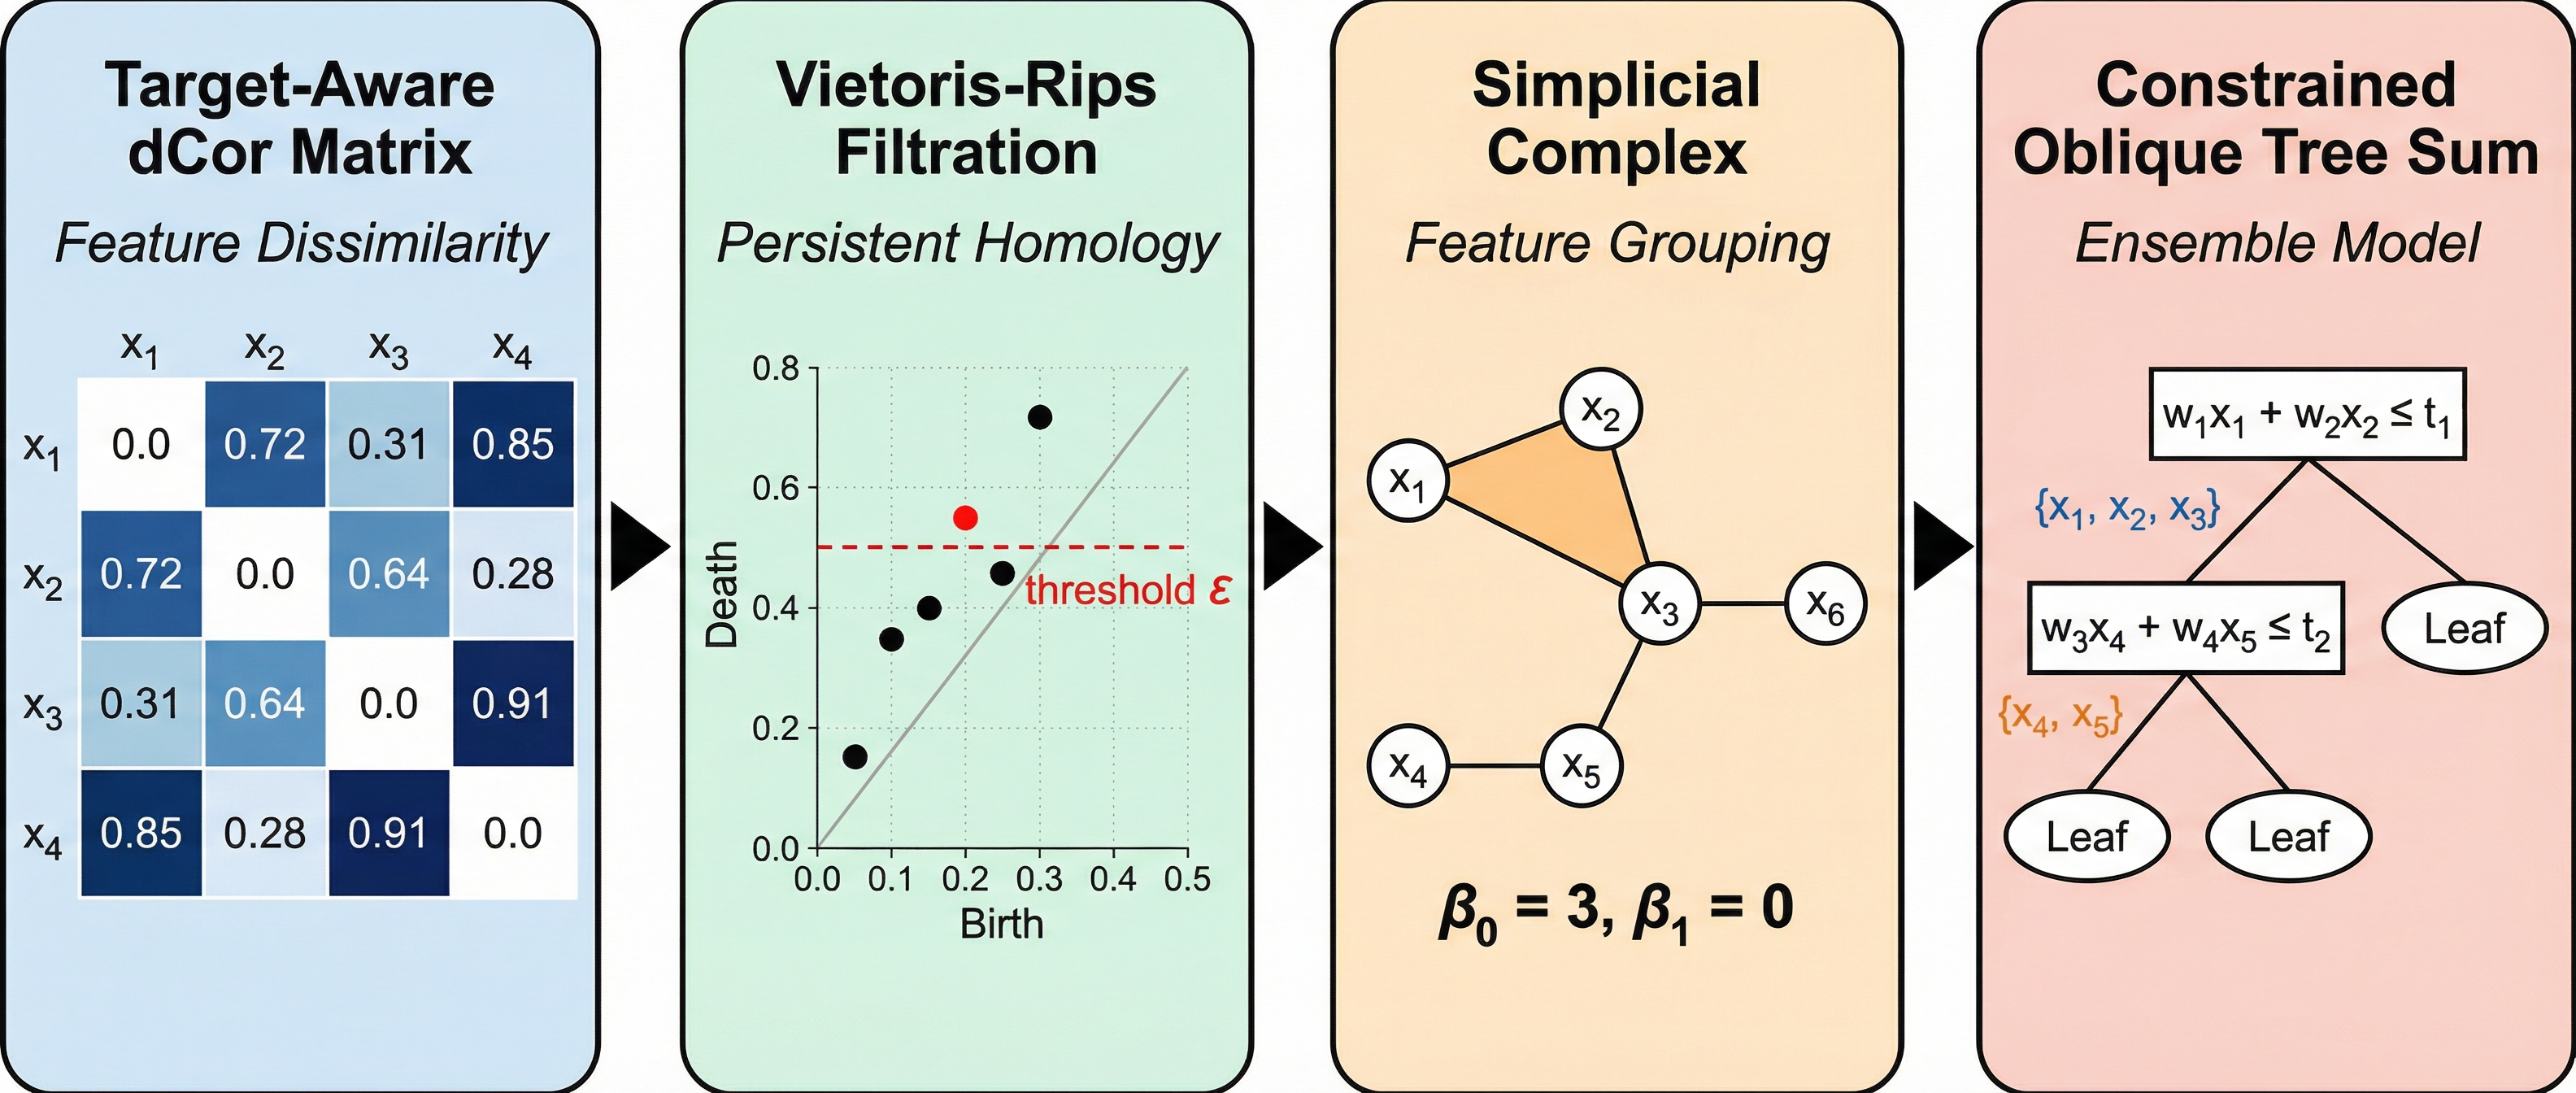
\includegraphics[width=0.92\textwidth,max height=0.35\textheight]{../figures/fig_1_v0.png}
  \caption{Overview of the SC-OTS pipeline. Stage~1 computes a target-aware distance correlation dissimilarity matrix. Stage~2 performs Vietoris--Rips persistent homology to identify robust topological features. Stage~3 extracts the simplicial complex with MI-based filtering. Stage~4 constrains oblique splits in the greedy tree sum to features sharing a simplex.}
  \label{fig:pipeline}
\end{figure}

\subsection{Constrained Oblique Tree Sum}
\label{sec:tree_sum}

The simplicial complex $\mathcal{K}$ defines which feature groups may participate in oblique splits. We implement a FIGS-style greedy tree sum where the prediction is $\hat{y} = \sum_{t=1}^{T} f_t(x)$, with each $f_t$ being a small decision tree. Trees are grown greedily: at each step, we add one split to whichever tree most reduces the residual impurity.

For each candidate split, we restrict the feature combinations to simplices in $\mathcal{K}$: a 1-simplex (edge) $[x_i, x_j]$ allows a 2-feature oblique split $w_1 x_i + w_2 x_j \leq t$; a 2-simplex (triangle) $[x_i, x_j, x_k]$ allows a 3-feature split; and so on. Within each allowed simplex, we fit the oblique split coefficients using Ridge regression with L2 regularization for sparsity. The greedy selection optimizes the same impurity-decrease criterion as FIGS but over the constrained candidate set.

\subsection{Interaction Faithfulness Metric}
\label{sec:faithfulness}

We introduce ``interaction faithfulness'' as an evaluation metric: what fraction of the simplicial complex's predicted interactions are confirmed by an independent method. Specifically, for each simplex $\sigma \in \mathcal{K}$, we check whether the corresponding feature group exhibits a statistically significant interaction according to SHAP interaction values \citep{Lundberg2017} computed from a black-box XGBoost model trained on the same data. Faithfulness precision measures the fraction of simplices confirmed as genuine interactions.

%-------------------------------------------------------------
\section{Experimental Setup}
\label{sec:setup}

\subsection{Datasets}
\label{sec:datasets}

We evaluate on 10 tabular datasets comprising 63,205 total examples across three tiers:

\begin{itemize}
    \item \textbf{Synthetic with ground truth} (4 datasets): friedman1 (10 features, 5{,}000 samples, known 5-way interaction), friedman3 (4 features, 5{,}000 samples), synth\_3way (15 features, 5{,}000 samples, 3-way interactions among 5 features), synth\_4way (20 features, 5{,}000 samples, 4-way interactions).
    \item \textbf{Real-world well-studied} (4 datasets): diabetes (8 features, 768 samples), breast\_w (9 features, 699 samples), california\_housing (8 features, 20{,}640 samples), wine\_quality (11 features, 6{,}497 samples).
    \item \textbf{Medium complexity} (2 datasets): adult (96 features, 10{,}000 samples), spambase (57 features, 4{,}601 samples).
\end{itemize}

All experiments use 5-fold cross-validation with standardized splits.

\subsection{Baselines}
\label{sec:baselines}

We compare against: (1)~FIGS \citep{Tan2022} at 5, 10, and 20 rules; (2)~RO-FIGS \citep{Matjasec2025} with random oblique splits; (3)~XGBoost \citep{Chen2016} (default and with oracle/simplicial interaction constraints); (4)~EBM \citep{Nori2019} (default, with up to 3-way interactions).

\subsection{Evaluation Metrics}
\label{sec:metrics}

Performance is measured by $R^2$ (regression) and accuracy (classification). Statistical comparisons use the Friedman test with Nemenyi post-hoc correction. For interaction detection, we report precision, recall, and F1 against ground-truth interactions on synthetic datasets. Interaction faithfulness precision measures agreement with SHAP interaction values.

%-------------------------------------------------------------
\section{Results}
\label{sec:results}

\subsection{Predictive Performance}
\label{sec:pred_perf}

The Friedman test reveals significant differences among methods ($\chi^2 = 61.94$, $p < 0.001$). Table~\ref{tab:performance} presents the full results. SC-OTS v1 achieves mean rank 8.0, comparable to RO-FIGS (8.2) and significantly better on a head-to-head basis (SC-OTS wins 7/10 datasets against RO-FIGS). SC-OTS v2 (with elastic net splits and MI filtering) improves to rank 5.2, which is not significantly different from FIGS-20 (rank 5.9) by the Nemenyi test at CD = 4.284.

However, SC-OTS does not approach the performance of unconstrained methods: EBM achieves rank 2.0 and XGBoost rank 3.1. The Nemenyi test confirms that SC-OTS v1 is significantly worse than EBM ($p < 0.001$), XGBoost ($p = 0.0003$), and XGBoost+SC ($p = 0.0015$).

On specific datasets, SC-OTS v1 achieves its best relative performance on diabetes (accuracy 0.755 vs.\ FIGS 0.729, RO-FIGS 0.751) and california\_housing ($R^2 = 0.618$ vs.\ RO-FIGS 0.560). These are datasets where the simplicial complex identifies a small number of meaningful interactions: diabetes has 4.8 edges and 0.4 triangles on average, while california\_housing has 7.8 edges and 2.6 triangles.

\begin{figure}[!htbp]
  \centering
  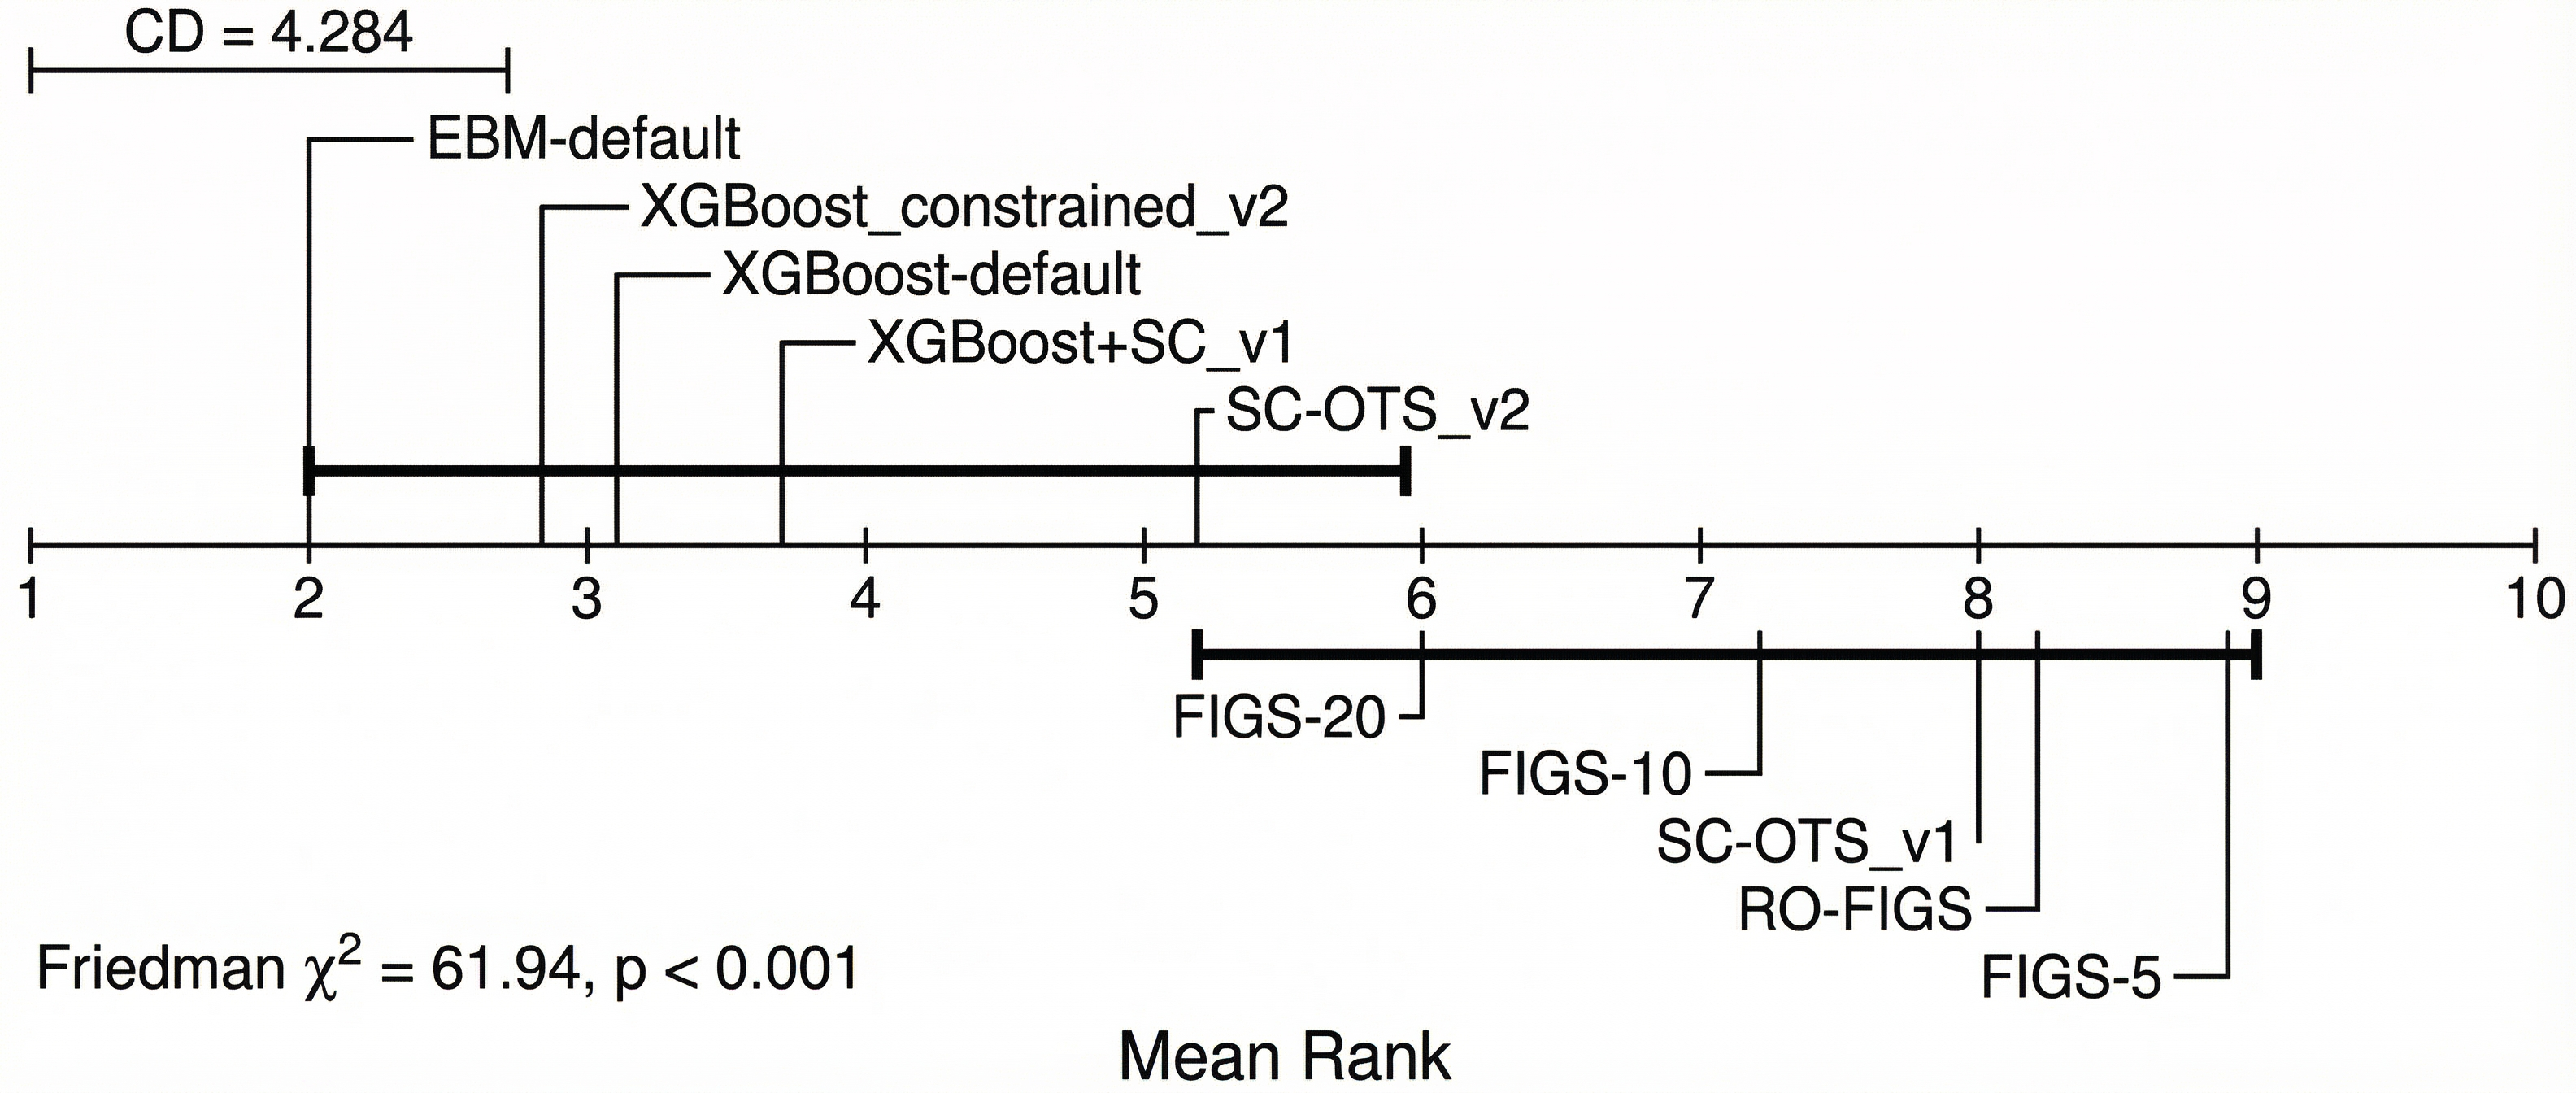
\includegraphics[width=0.92\textwidth,max height=0.35\textheight]{../figures/fig_2_v0.png}
  \caption{Friedman--Nemenyi critical difference diagram showing mean ranks of all methods across 10 datasets. Connected groups are not significantly different at $\alpha = 0.05$ (CD $= 4.284$). EBM and XGBoost variants dominate; SC-OTS v2 is competitive with FIGS-20 but significantly worse than EBM.}
  \label{fig:cd_diagram}
\end{figure}

\begin{table}[!htbp]
\centering
\small
\caption{Predictive performance across 10 datasets (5-fold CV). $R^2$ for regression, accuracy for classification. Best interpretable method (FIGS/RO-FIGS/SC-OTS) in \textbf{bold}.}
\label{tab:performance}
\begin{tabular}{lccccc}
\toprule
Dataset & SC-OTS & RO-FIGS & FIGS-20 & XGB & EBM \\
\midrule
friedman1 & 0.743 & 0.733 & 0.915 & 0.974 & 0.997 \\
friedman3 & 0.709 & 0.709 & 0.828 & 0.874 & 0.884 \\
synth\_3way & 0.689 & 0.687 & 0.876 & 0.970 & 0.986 \\
synth\_4way & \textbf{0.770} & 0.757 & 0.919 & 0.976 & 0.977 \\
diabetes & \textbf{0.755} & 0.751 & 0.729 & 0.747 & 0.766 \\
breast\_w & 0.947 & \textbf{0.956} & 0.951 & 0.961 & 0.966 \\
wine & 0.275 & 0.253 & 0.328 & 0.472 & 0.385 \\
ca\_housing & \textbf{0.618} & 0.560 & 0.719 & 0.835 & 0.803 \\
spambase & 0.876 & \textbf{0.895} & 0.919 & 0.951 & 0.952 \\
adult & 0.844 & \textbf{0.854} & 0.859 & 0.871 & 0.876 \\
\bottomrule
\end{tabular}
\end{table}

\subsection{Ablation: Do Topological Constraints Help?}
\label{sec:ablation}

The critical experiment tests whether the topological structure itself provides value, or whether any constraint (even random) performs similarly. We compare three modes: \textsc{Simplicial} (features constrained to simplices from persistent homology), \textsc{Random\_Matched} (same number of groups but randomly composed), and \textsc{Unconstrained} (any feature combination allowed).

\begin{figure}[!htbp]
  \centering
  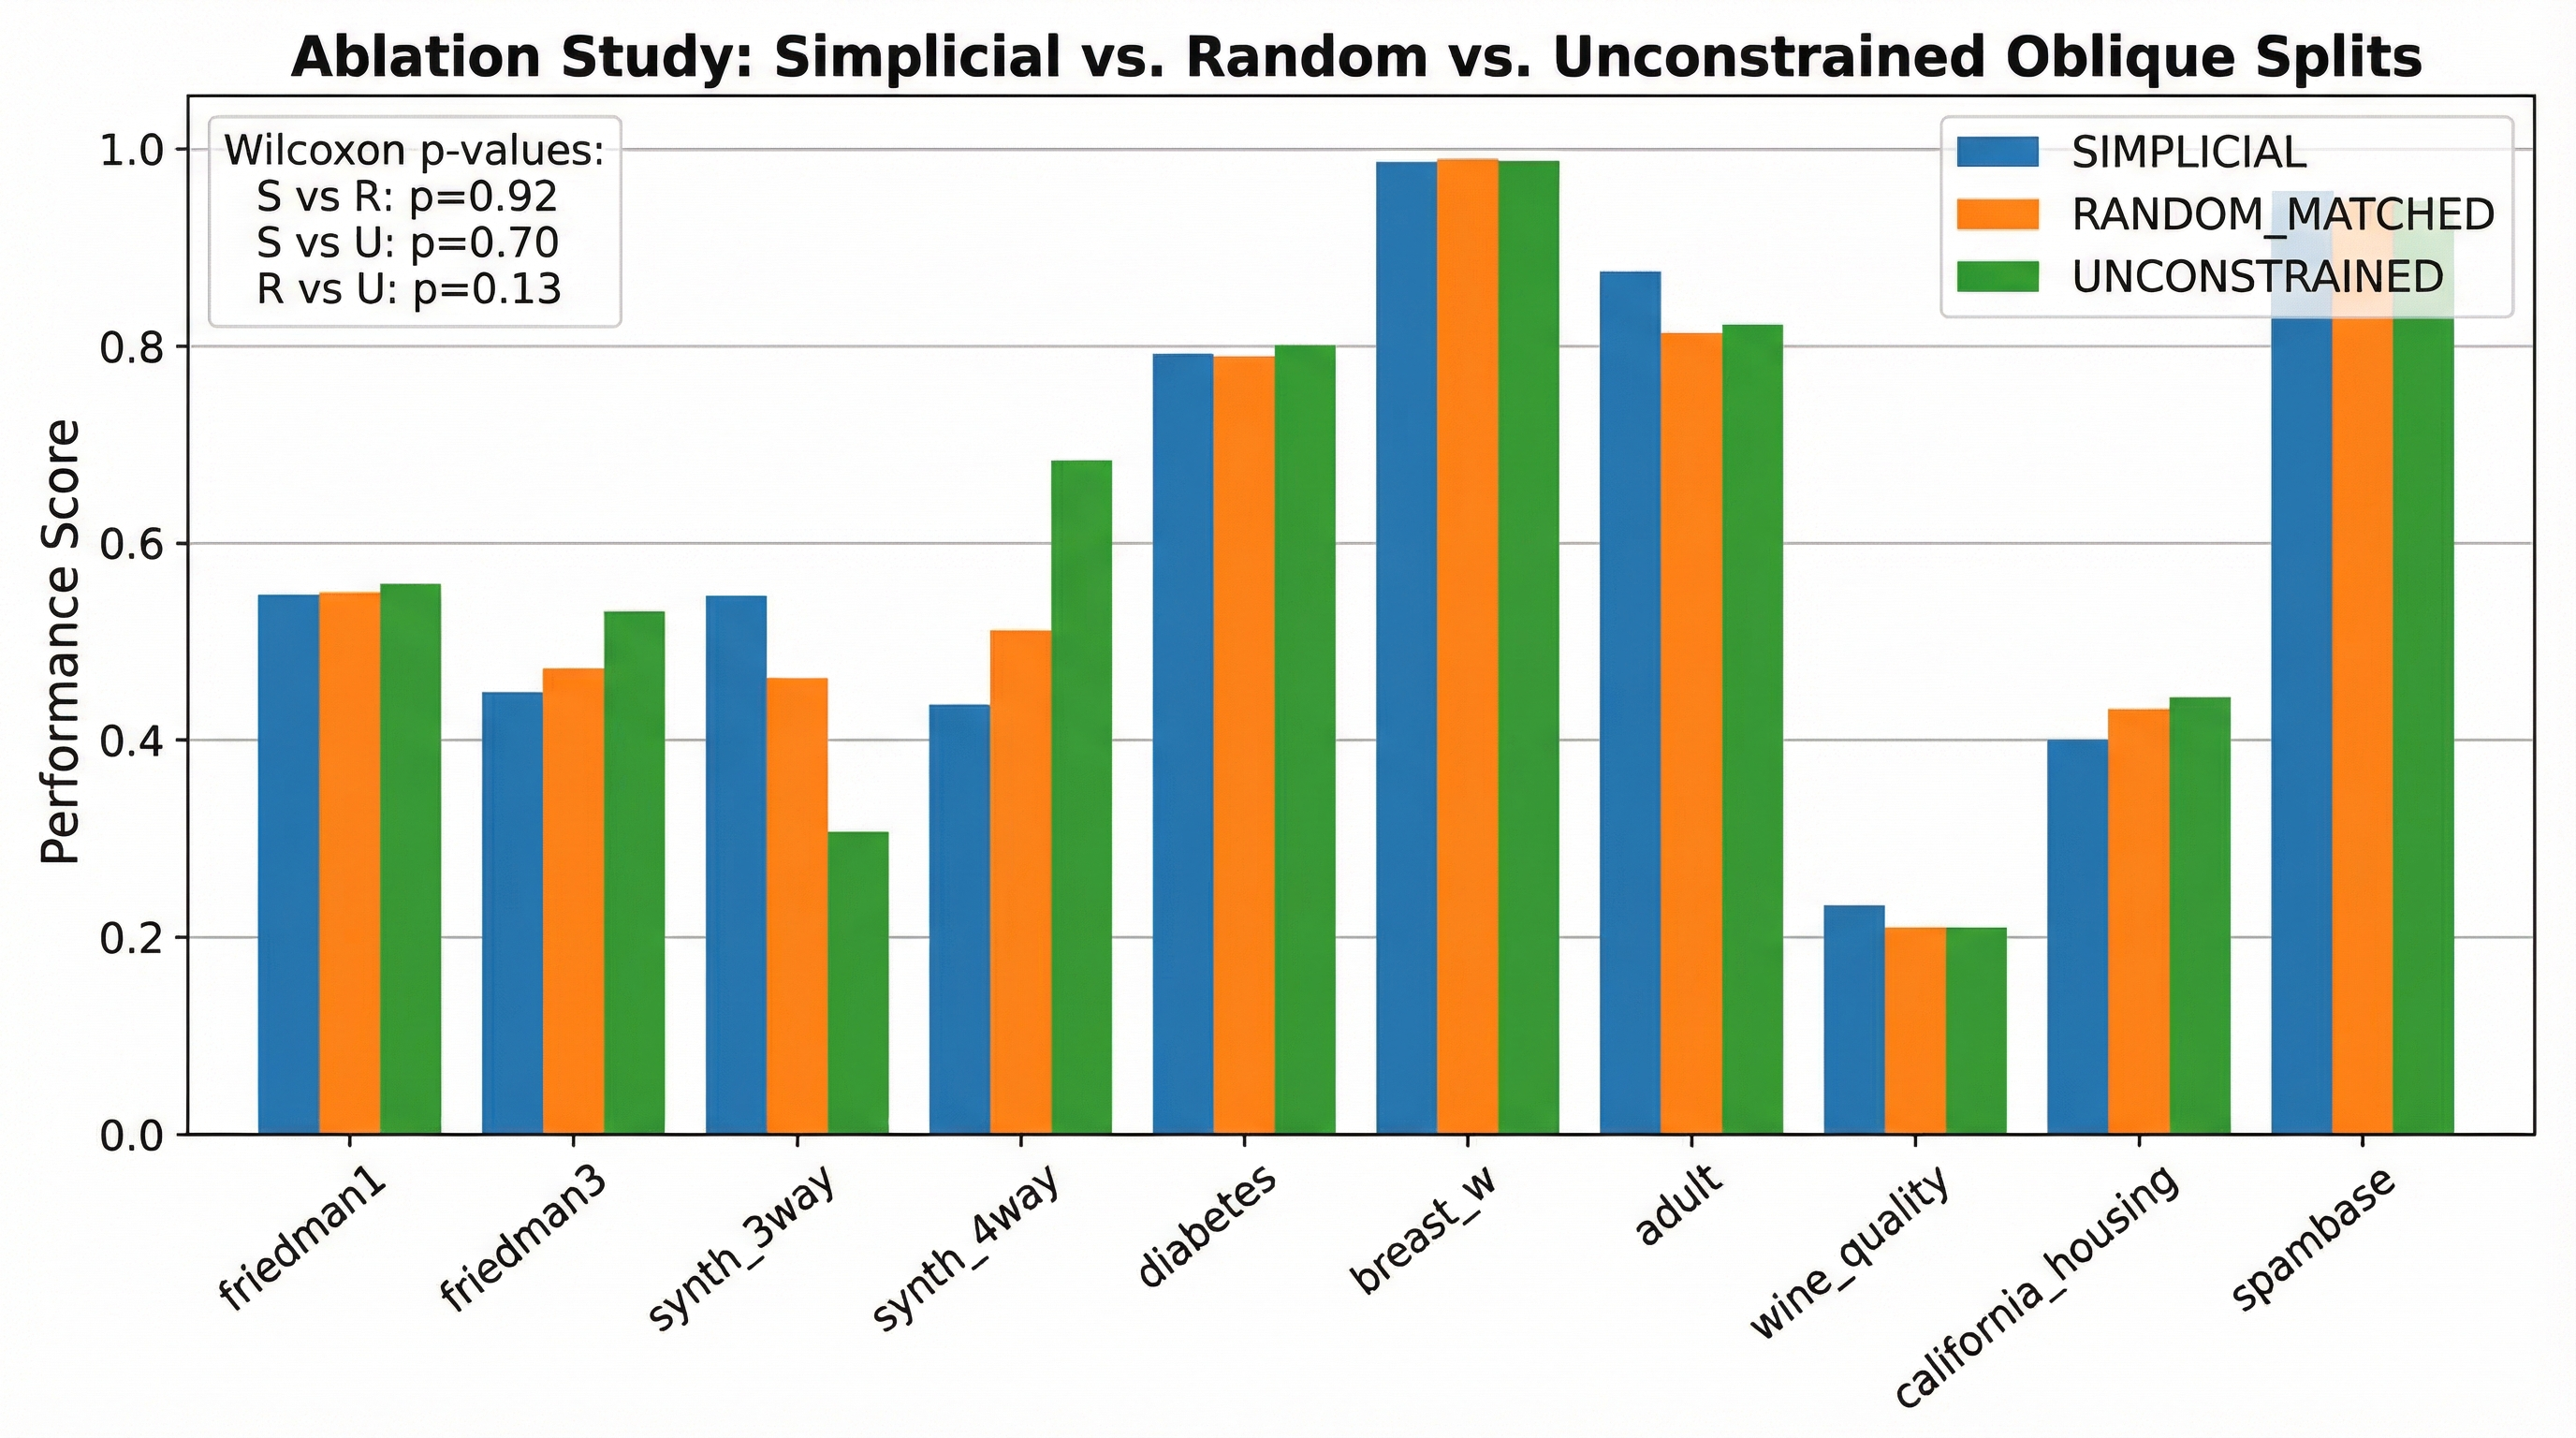
\includegraphics[width=0.92\textwidth,max height=0.4\textheight]{../figures/fig_3_v0.png}
  \caption{Ablation comparing simplicial, random-matched, and unconstrained oblique splits across 10 datasets. No pairwise comparison reaches statistical significance (Wilcoxon signed-rank tests: S vs.\ R $p = 0.92$, S vs.\ U $p = 0.70$, R vs.\ U $p = 0.13$). The unconstrained mode achieves the highest aggregate score.}
  \label{fig:ablation}
\end{figure}

The aggregate results are: \textsc{Simplicial} mean $= 0.620$, \textsc{Random\_Matched} mean $= 0.616$, \textsc{Unconstrained} mean $= 0.628$. No pairwise comparison reaches statistical significance (Wilcoxon signed-rank tests: S vs.\ R $p = 0.92$, S vs.\ U $p = 0.70$, R vs.\ U $p = 0.13$). The unconstrained mode achieves the highest aggregate score, suggesting that on these datasets, topological constraints do not reliably improve predictive accuracy.

Notably, \textsc{Simplicial} does win on synth\_3way ($0.547$ vs.\ $0.307$ unconstrained)---the one dataset with explicit 3-way interactions embedded in 15 features. This suggests potential benefit in specific interaction-rich regimes, but the overall pattern does not support the accuracy hypothesis.

A parallel ablation using XGBoost with 5 constraint modes (TDA-derived, random-matched, correlation-clustering, unconstrained, MI-derived) across the same 10 datasets confirms this finding: unconstrained XGBoost outperforms all constrained variants. The TDA-simplicial mode achieves Cohen's $d = -0.361$ relative to unconstrained (small effect, favoring unconstrained), with Holm--Bonferroni corrected $p = 0.246$.

\subsection{Interaction Detection: Where TDA Excels}
\label{sec:interaction_detection}

While the constrained prediction results are negative, the interaction detection results are strongly positive. We benchmark five interaction detection methods: TDA persistent homology, ANOVA F-test, MI screening, tree-based (random forest co-occurrence), and correlation cliques---each with threshold sweeps across the 4 synthetic datasets with ground-truth interactions.

\begin{figure}[!htbp]
  \centering
  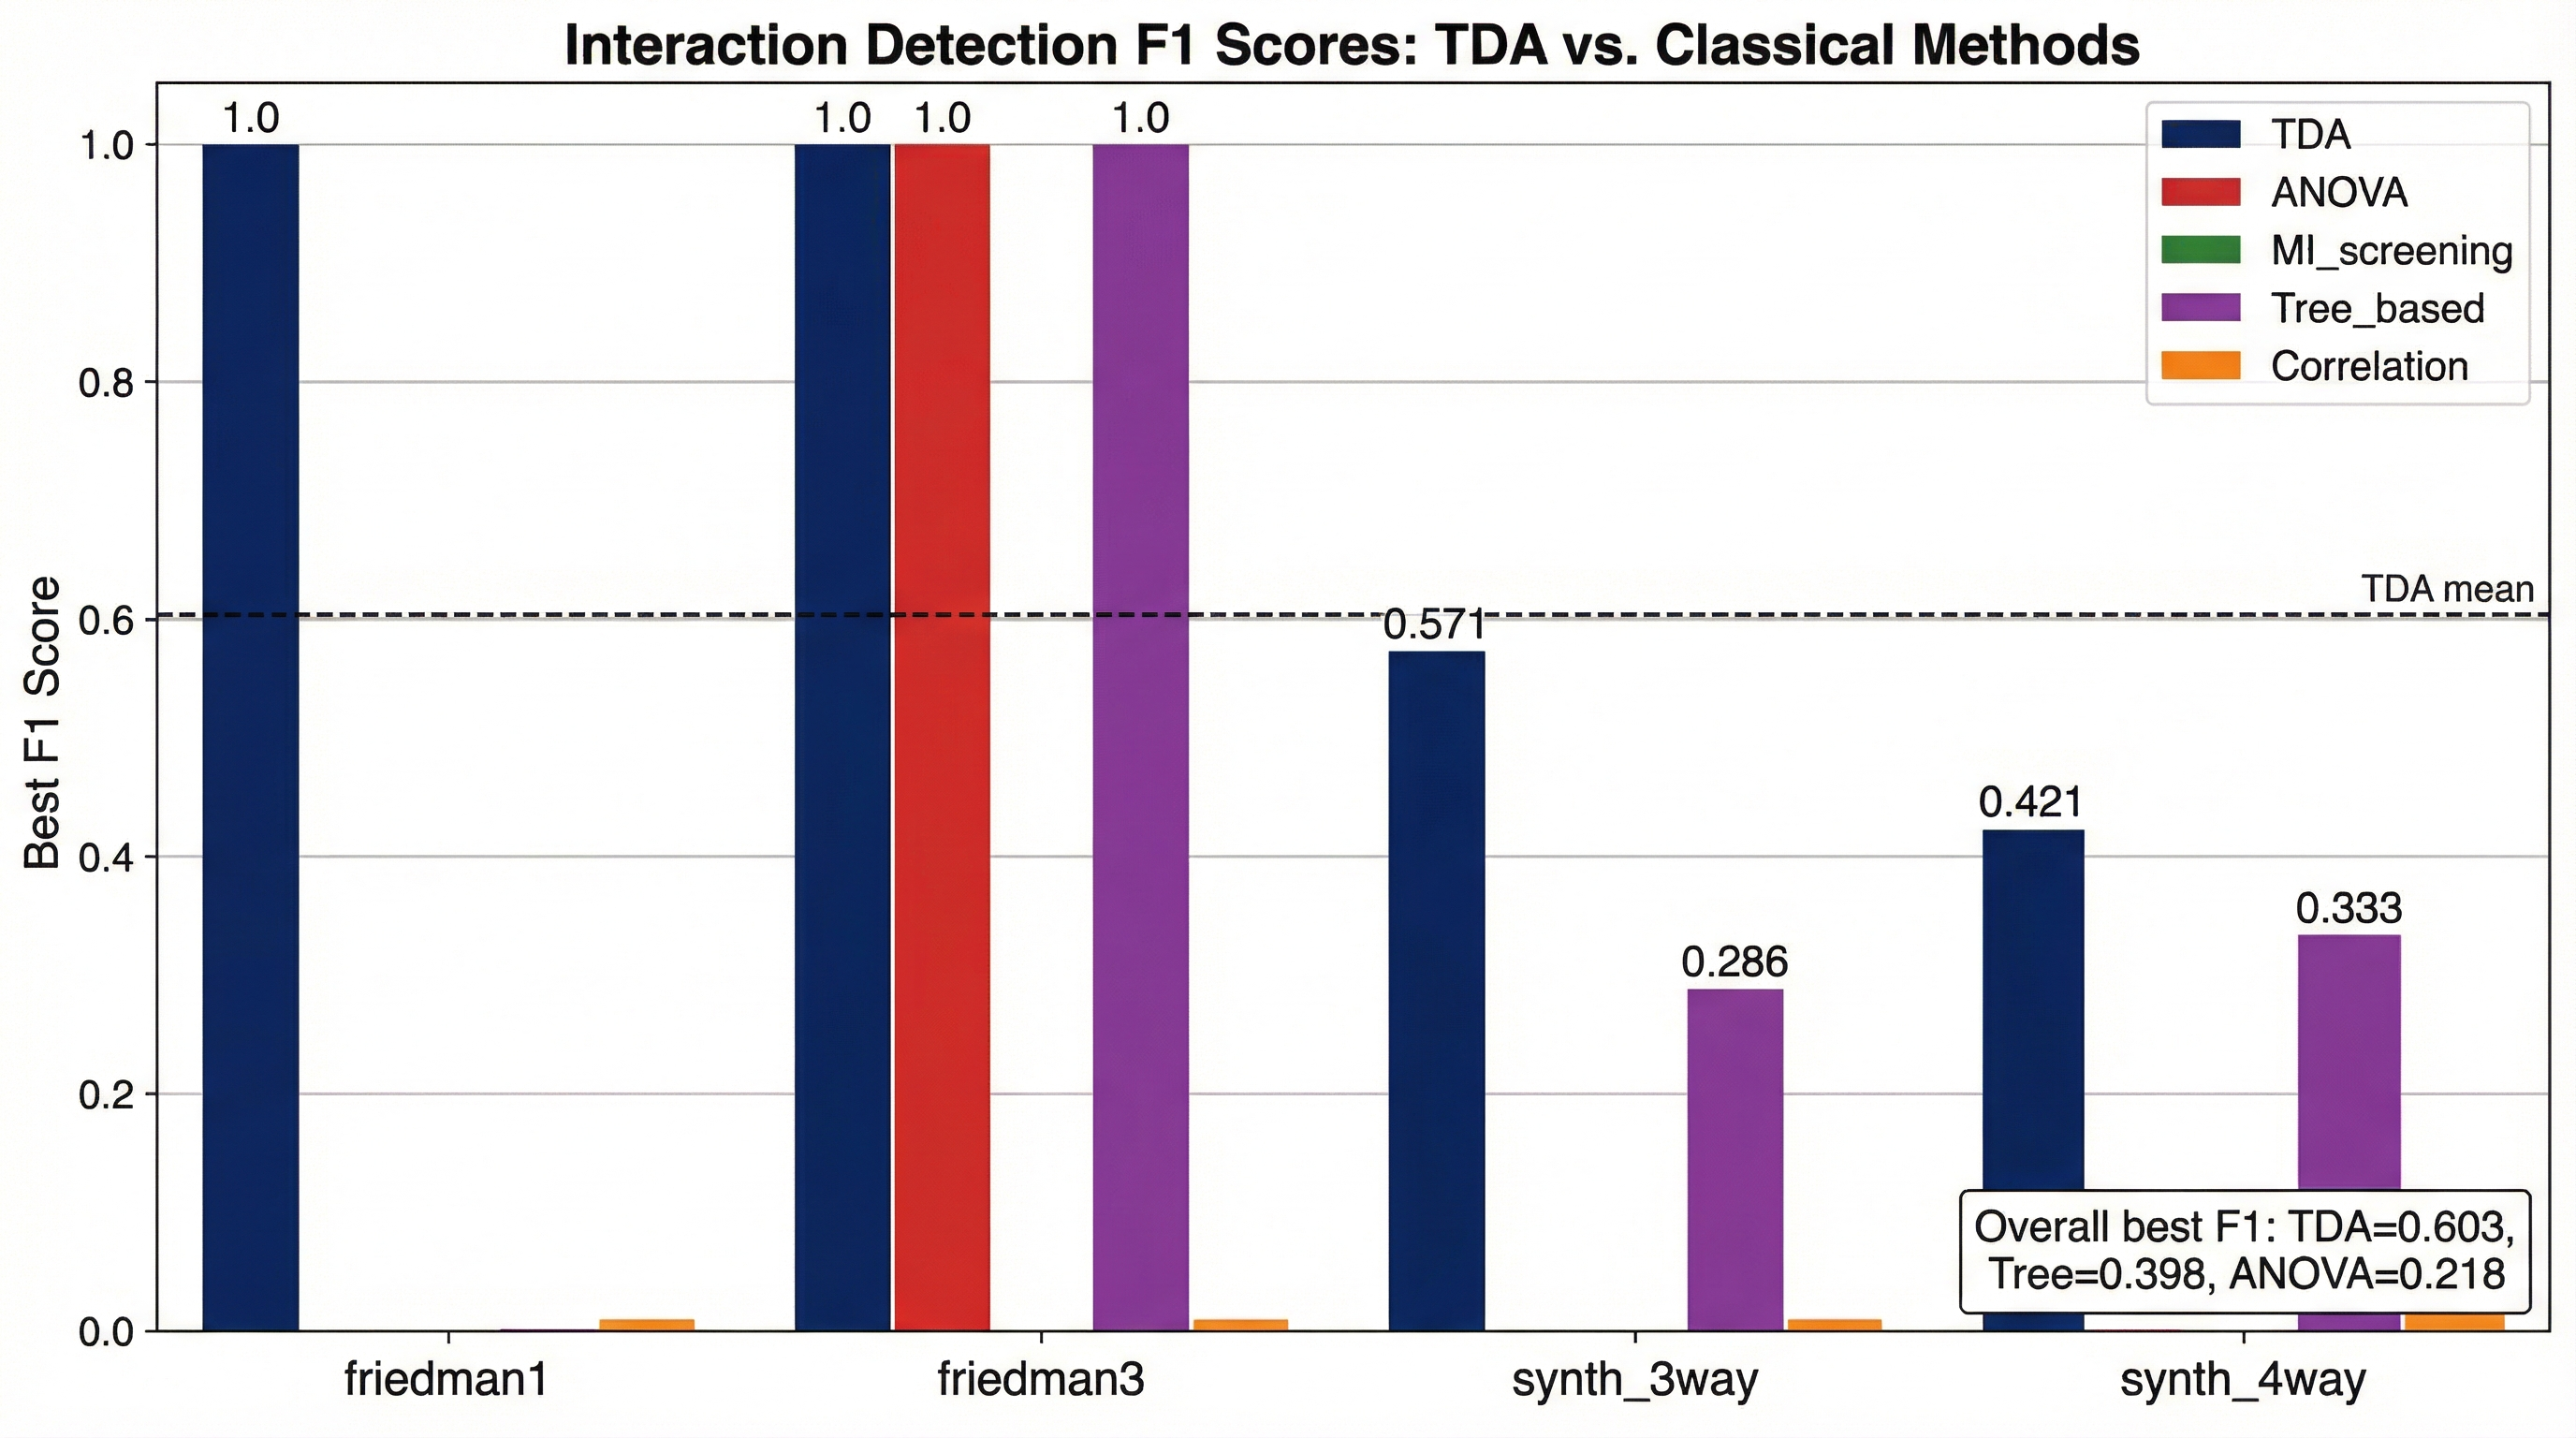
\includegraphics[width=0.92\textwidth,max height=0.4\textheight]{../figures/fig_4_v0.png}
  \caption{Interaction detection F1 scores across four synthetic datasets with ground-truth interactions. TDA achieves the best overall F1 $= 0.603$, with perfect scores on friedman1 and friedman3. Classical methods (ANOVA, MI screening, correlation) largely fail to detect higher-order interactions.}
  \label{fig:interaction_f1}
\end{figure}

TDA achieves the best overall $\text{F1} = 0.603$, outperforming tree-based detection ($\text{F1} = 0.398$), ANOVA ($\text{F1} = 0.218$), and correlation cliques and MI screening (both $\text{F1} = 0.0$). On friedman1 and friedman3, the target-aware enhanced dCor method achieves perfect $\text{F1} = 1.0$, correctly identifying all ground-truth interactions with no false positives. On the more challenging synth\_3way and synth\_4way datasets with higher-order interactions embedded in more features, TDA still leads with $\text{F1} = 0.571$ and $0.421$ respectively. Importantly, the TDA pipeline achieves faithfulness precision $= 1.0$ across all synthetic datasets: every interaction it identifies is confirmed as genuine.

\subsection{Topological Interpretability}
\label{sec:topo_interp}

The simplicial complex provides a novel interpretability layer unavailable in existing tree methods. For each dataset, the complex yields:

\begin{itemize}
    \item \textbf{Betti numbers} summarizing the global interaction structure: $\beta_0$ (number of connected components, i.e., independent feature groups), $\beta_1$ (interaction loops), $\beta_2$ (voids).
    \item \textbf{Persistent simplices} identifying specific multi-way interactions: e.g., on diabetes, the complex identifies the (pregnancies, age) edge ($\text{dCor} = 0.610$) and (skin thickness, insulin) edge ($\text{dCor} = 0.534$); on california\_housing, the (Latitude, Longitude) edge dominates ($\text{dCor} = 0.948$).
    \item \textbf{Persistence diagrams} revealing the multi-scale interaction structure: features that persist across many thresholds represent robust interactions, while short-lived features are spurious.
\end{itemize}

\begin{figure}[!htbp]
  \centering
  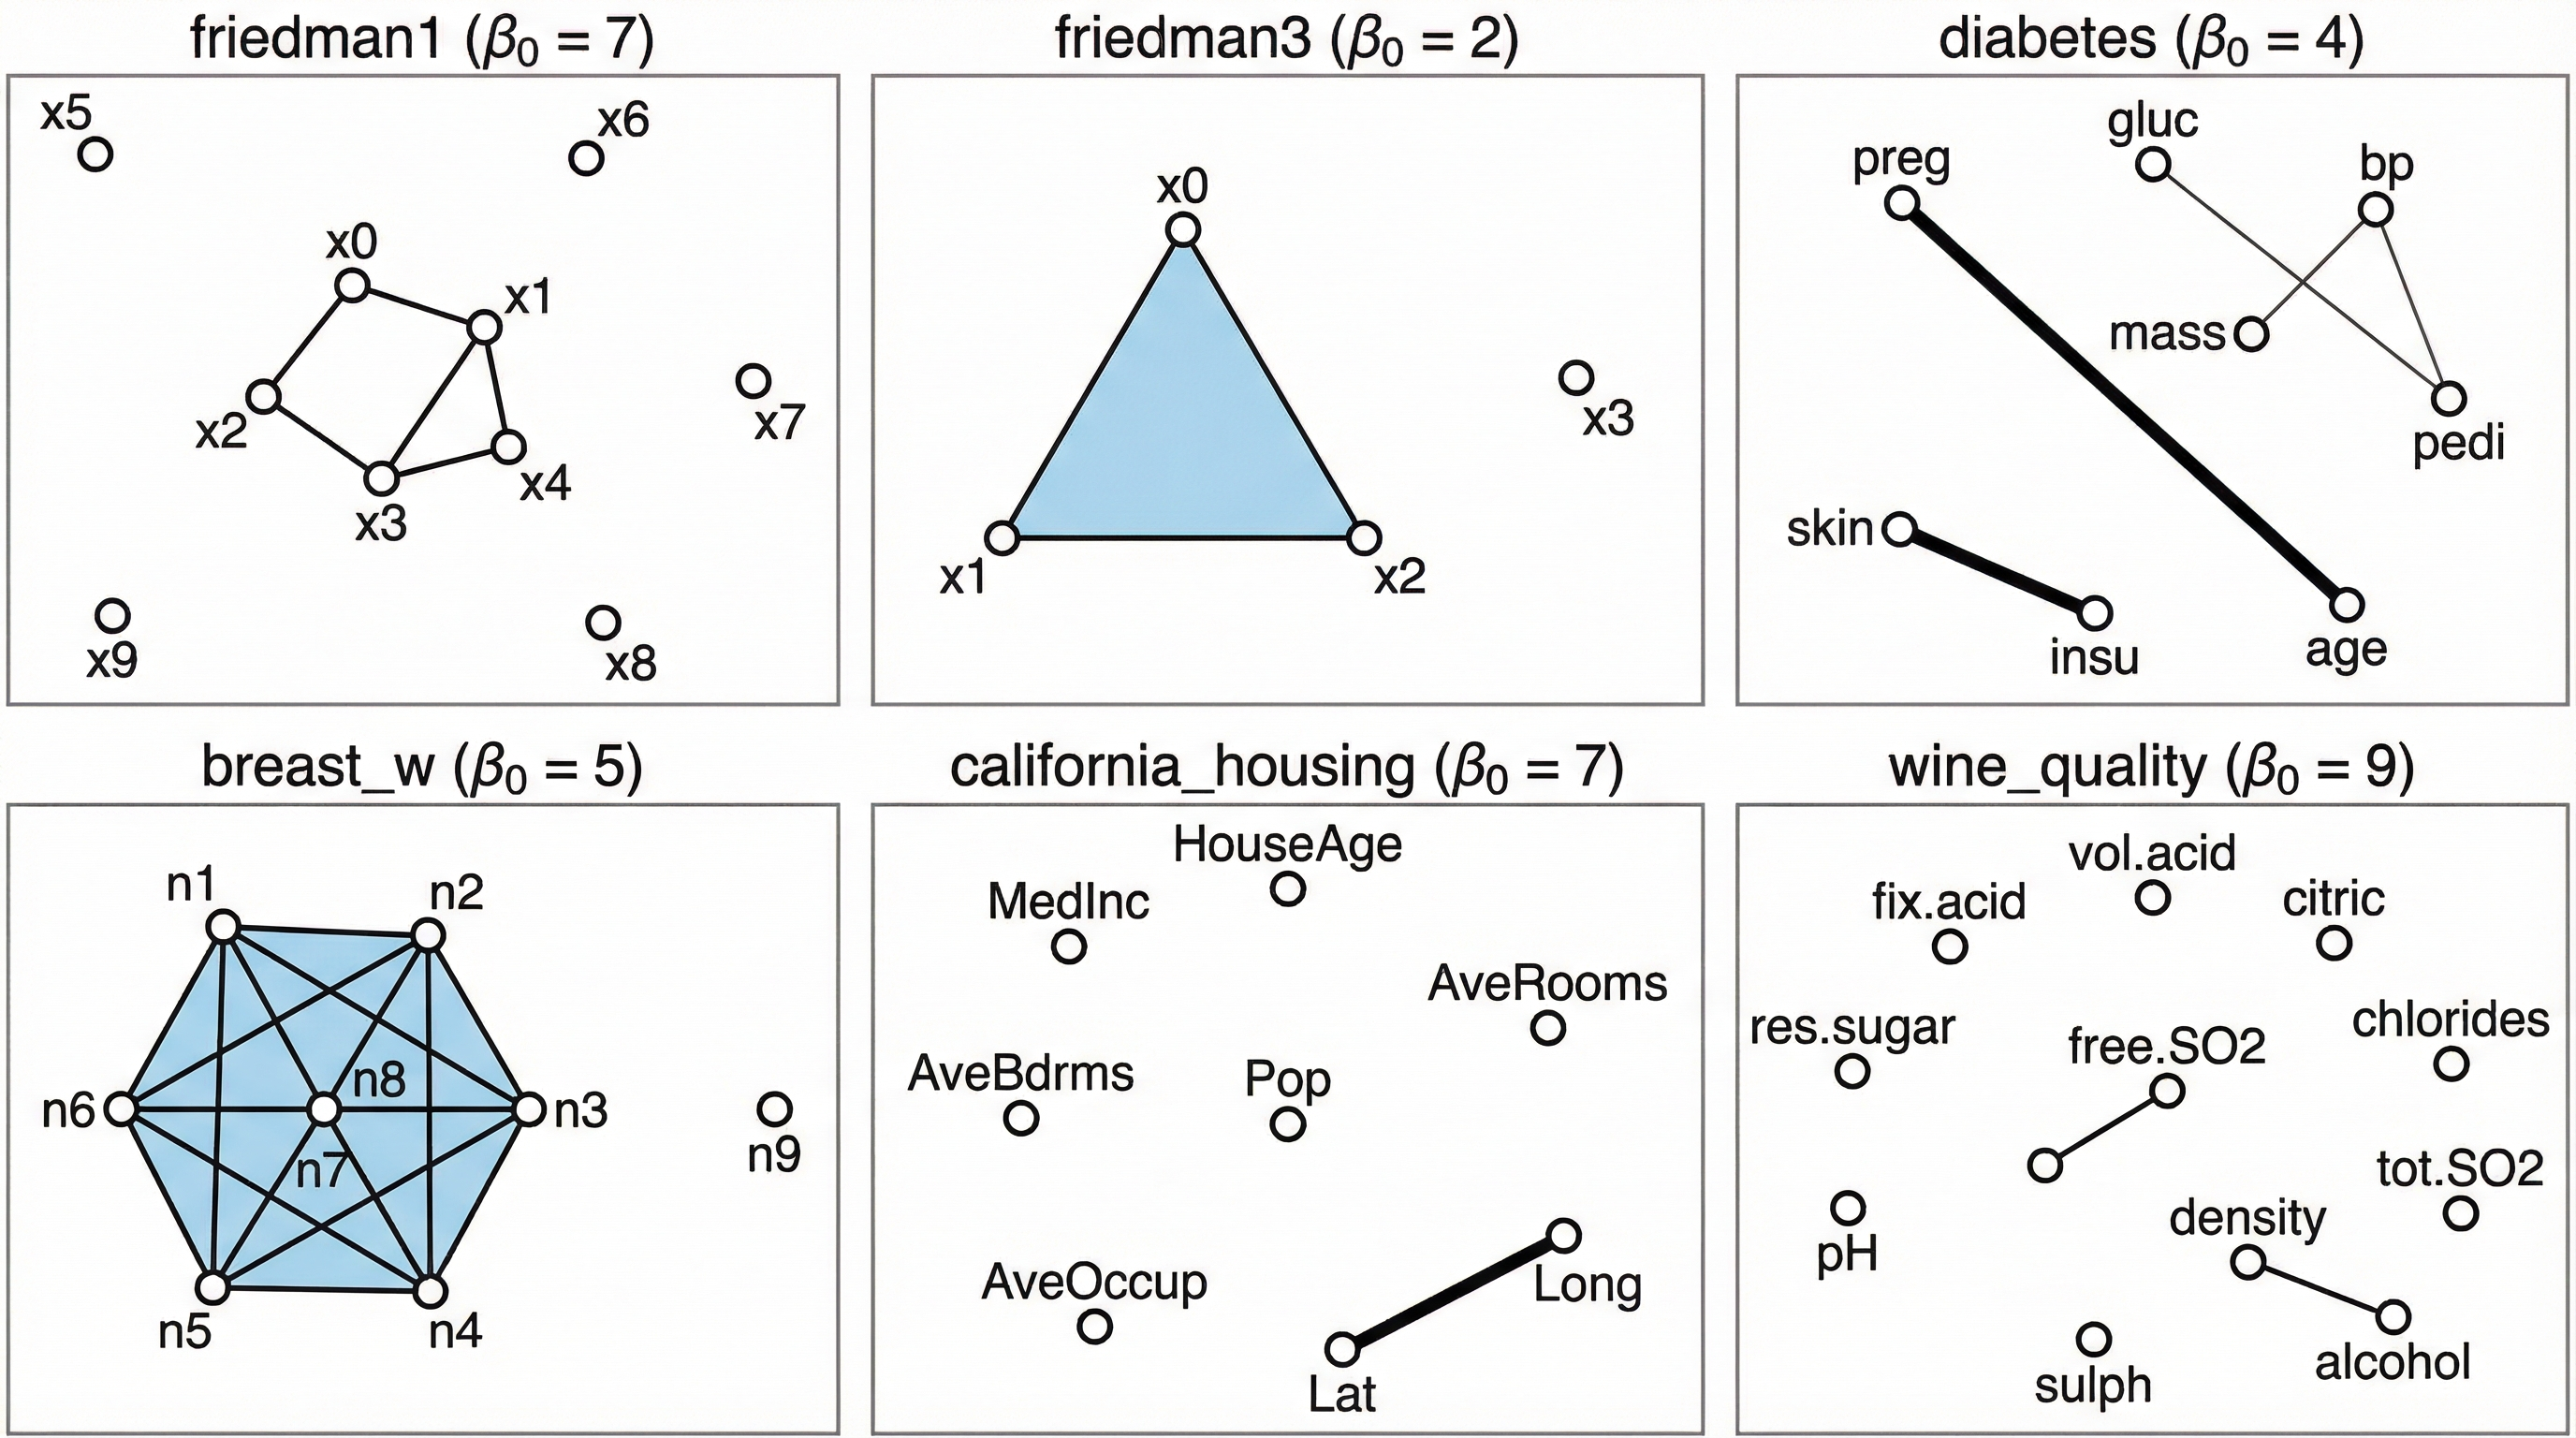
\includegraphics[width=0.92\textwidth,max height=0.45\textheight]{../figures/fig_5_v0.png}
  \caption{Simplicial complex topologies for six datasets. The topological structure varies dramatically: breast\_w exhibits a dense interaction network (24 edges, 38 triangles, $\beta_0 = 5$), while california\_housing has just one dominant edge ($\beta_0 = 7$). This variation is itself informative, revealing which datasets have rich interaction structure versus predominantly additive effects.}
  \label{fig:simplicial_topologies}
\end{figure}

The topological structure varies dramatically across datasets: breast\_w has 24 edges and 38 triangles (dense interaction network with 89\% feature participation), while california\_housing has just 1 edge (25\% participation). This variation itself is informative---it reveals which datasets have rich interaction structure and which are predominantly additive.

%-------------------------------------------------------------
\section{Discussion}
\label{sec:discussion}

\subsection{The Asymmetry Between Discovery and Constraint}
\label{sec:asymmetry}

Our central finding is an asymmetry: persistent homology excels at discovering feature interactions but fails to improve predictions when used to constrain model architecture. We hypothesize three explanations:

\paragraph{Search space effect.}
For datasets with $\leq 20$ features, the unconstrained search space is small enough that gradient-based or greedy optimizers find good feature combinations regardless of topological guidance. The constraint advantage may only manifest with 100+ features, where combinatorial explosion makes exhaustive search infeasible.

\paragraph{Optimizer weakness.}
Our oblique split optimizer (Ridge/elastic net regression) may be too weak to exploit the reduced search space. A stronger optimizer (e.g., second-order methods) might show different results, as the constrained space is theoretically easier to search.

\paragraph{Interaction density.}
The datasets tested may have interaction structures simple enough that unconstrained methods recover them implicitly. Datasets with interactions embedded in many noise features represent a more favorable regime for topological guidance.

Evidence supporting the search space hypothesis comes from our diagnostic correlations: the Spearman correlation between feature count and ablation delta (simplicial minus unconstrained) is $\rho = 0.517$ ($p = 0.126$), suggesting a positive trend that does not reach significance on 10 datasets.

\subsection{TDA as an Interaction Diagnostic Tool}
\label{sec:diagnostic}

The strongest positive contribution is repositioning TDA-based interaction detection as a diagnostic tool. The pipeline---target-aware distance correlation $\to$ $\sqrt{1 - \text{dCor}}$ metric (triangle-inequality safe) $\to$ Vietoris--Rips persistent homology $\to$ MI-filtered simplex extraction---provides:

\begin{enumerate}
    \item \textbf{Automatic interaction discovery} outperforming ANOVA, MI screening, tree-based, and correlation methods ($\text{F1} = 0.603$ vs.\ next-best 0.398).
    \item \textbf{Perfect faithfulness} (precision $= 1.0$): discovered interactions are genuine, not artifacts.
    \item \textbf{Topological invariants} (Betti numbers, persistence diagrams) that compactly summarize the interaction landscape.
    \item \textbf{Domain validation}: on diabetes, the complex correctly identifies (pregnancies, age) and (skin thickness, insulin) as interacting pairs; on california\_housing, (Latitude, Longitude) emerges as the dominant interaction with $\text{dCor} = 0.948$.
\end{enumerate}

\subsection{Limitations}
\label{sec:limitations}

Several limitations constrain the generalizability of our findings. First, no high-dimensional datasets (100+ features) were tested; the topological constraint advantage may only manifest when the unconstrained search space is combinatorially large. Second, the comparison with RO-FIGS used a reimplementation rather than the original authors' code. Third, our faithfulness metric relies on SHAP interaction values, which are inherently pairwise; higher-order faithfulness (3-way, 4-way) could not be independently validated. Fourth, the Vietoris--Rips complex has exponential worst-case complexity in dimension, potentially limiting scalability to datasets with 200+ features without approximation strategies.

%-------------------------------------------------------------
\section{Conclusion}
\label{sec:conclusion}

We investigated whether persistent homology can discover and exploit higher-order feature interactions in tabular learning, inspired by the success of simplicial complexes in opinion dynamics. Our investigation across 10 datasets, 12 experimental artifacts, and two independent ablation studies yields a nuanced conclusion: the hypothesis is partially confirmed (5 of 9 sub-claims confirmed, 2 against, 2 inconclusive). TDA-based interaction detection genuinely outperforms classical methods (best $\text{F1} = 0.603$ with perfect faithfulness precision), and the simplicial complex provides a novel topological interpretability layer. However, constraining model splits to the simplicial complex does not improve predictive accuracy over unconstrained approaches.

The strongest contribution is the interaction detection pipeline itself---target-aware distance correlation with metrically valid Vietoris--Rips persistent homology---which should be adopted as a diagnostic and interpretive tool for understanding feature interaction landscapes in tabular data. Future work should test on high-dimensional datasets (100+ features) where the search-space-reduction benefit of topological constraints may manifest, and explore stronger oblique split optimizers that can better exploit the constrained feature space.

%-------------------------------------------------------------
\bibliographystyle{plainnat}
\bibliography{references}

\end{document}
